\documentclass[varwidth=true, border=2pt]{standalone}
\usepackage{tikz}
\usetikzlibrary{shapes, calc, shapes, arrows, decorations.markings}
\usepackage{amsmath,amssymb}

\usepackage{xcolor}
\definecolor{xvectorcolor}{HTML}{77933C}

\begin{document}
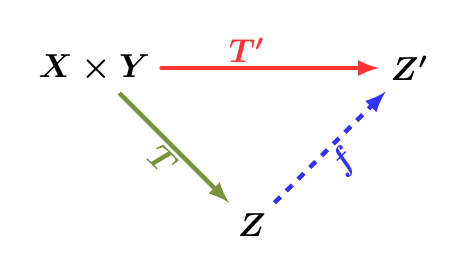
\begin{tikzpicture}[font=\boldmath]
    \large

    % Points
    \node (A) at (0,2) {$X \times Y$};
    \node (B) at (4,2) {$Z'$};
    \node (C) at (2,0) {$Z$};

    % Round loop arrow in middle:
    %\draw[->, ultra thick] (2.1,0.7) arc(-70:260:0.4);

    \draw[ultra thick,xvectorcolor,         arrows={-latex}]  (A) -- (C) node[sloped,midway,below=-0.1cm] {$T$};
    \draw[ultra thick,blue!80, dashed,      arrows={-latex}]  (C) -- (B) node[sloped,midway,below=-0.1cm] {$f$};
    \draw[ultra thick,red!80,line cap=round,arrows={-latex}]  (A) -- (B) node[sloped,midway,right=-0.3cm,above=-0.1cm] {$T'$};
\end{tikzpicture}
\end{document}
